%%% LaTeX Template
%%% This template can be used for both articles and reports.
%%%
%%% Copyright: http://www.howtotex.com/
%%% Date: February 2011

%%% Preamble
\documentclass[paper=a4, fontsize=11pt]{scrartcl}	% Article class of KOMA-script with 11pt font and a4 format
\usepackage[margin=0.7in]{geometry}
\usepackage[english]{babel}															% English language/hyphenation
\usepackage[protrusion=true,expansion=true]{microtype}				% Better typography
\usepackage{amsmath,amsfonts,amsthm}										% Math packages
%\usepackage{color,transparent}													% If you use color and/or transparency
\usepackage[hang, small,labelfont=bf,up,textfont=it,up]{caption}	% Custom captions under/above floats
\usepackage{epstopdf}																	% Converts .eps to .pdf
\usepackage{subfig}																		% Subfigures
\usepackage{booktabs}																	% Nicer tables
\usepackage[pdftex]{graphicx}

%%% Advanced verbatim environment
\usepackage{verbatim}
\usepackage{fancyvrb}
\DefineShortVerb{\|}								% delimiter to display inline verbatim text


%%% Custom sectioning (sectsty package)
\usepackage{sectsty}								% Custom sectioning (see below)
\allsectionsfont{%									% Change font of al section commands
	\usefont{OT1}{bch}{b}{n}%					% bch-b-n: CharterBT-Bold font
%	\hspace{15pt}%									% Uncomment for indentation
	}

\sectionfont{%										% Change font of \section command
	\usefont{OT1}{bch}{b}{n}%					% bch-b-n: CharterBT-Bold font
	\sectionrule{0pt}{0pt}{-5pt}{0.8pt}%	% Horizontal rule below section
	}


%%% Custom headers/footers (fancyhdr package)
\usepackage{fancyhdr}
\pagestyle{fancyplain}
\fancyhead{}														% No page header
\fancyfoot[C]{\thepage}										% Pagenumbering at center of footer
\renewcommand{\headrulewidth}{0pt}				% Remove header underlines
\renewcommand{\footrulewidth}{0pt}				% Remove footer underlines
\setlength{\headheight}{13.6pt}

%%% Equation and float numbering
\numberwithin{equation}{section}															% Equationnumbering: section.eq#
\numberwithin{figure}{section}																% Figurenumbering: section.fig#
\numberwithin{table}{section}

\usepackage[parfill]{parskip}
\usepackage{float}
\usepackage{hyperref}
\usepackage[numbers]{natbib}															% Tablenumbering: section.tab#


%%% Title
\title{
	\vspace{-1in} 	\usefont{OT1}{bch}{b}{n}
	\huge \strut Industrial Year Report \strut \\
	\Large \bfseries \strut Software Developer at ISIS Neutron Source \strut
}

%% Authors
\author{
	\usefont{OT1}{bch}{m}{n} Samuel Jackson
	\\ \usefont{OT1}{bch}{m}{n} University Of Aberystwyth
	\\   \texttt{slj11@aber.ac.uk}
}

\date{\today}

\begin{document}
	\maketitle
	\clearpage
	\tableofcontents
	\clearpage
	\hyperdef{}{introduction}{\section{Introduction}\label{introduction}}

This report details the industrial placement year I undertook as part of
the Software Engineering MEng course at Aberystwyth university. The
position of the placement was a junior role as part of the Mantid data
analysis toolkit development team based at the ISIS facility at
Rutherford Appleton Laboratory in Harwell, Oxfordshire, which is owned
by the Science and Technologies Facilities Council (STFC). I held this
post for a total duration of 14 months, with 12 months on the original
contract and a 2 month extension.

ISIS is a world leading neutron and muon scattering facility. The
facility operates two target stations and a 800 MeV pulsed proton
synchrotron which acts as a source of neutrons for both neutron and muon
time-of-flight spectroscopy {[}1{]}. Neutron and muon spectroscopy is
used to probe the structure and dynamics of materials at the atomic
level.

The Mantid project {[}2{]} is a free, open source application which aims
to provide a single, unified application for the analysis of neutron and
muon scattering data from facilities such as ISIS. The project is
primarily developed by two teams of developers, one based at ISIS and
one at the Spallation Neutron Source (SNS) at Oakridge laboratory in
Tennessee, USA.

\subsection{Introduction to Neutron
Scattering}\label{introduction-to-neutron-scattering}

In order to fully understand the operation of ISIS and what the Mantid
application is used to analyse, a small amount of background knowledge
of the techniques used in neutron scattering experiments is useful along
with some definitions of key terms used through out this document.

Instruments at the ISIS facility are designed to probe the structure and
dynamics of materials at the atomic scale. ISIS operates by accelerating
protons to 84\% the speed of light using a synchrotron. The resulting
particles are then directed towards a tungsten target in one of the two
target stations causing a pulsed burst of neutrons which are directed
towards samples in the spectrometers. The resulting collisions cause a
scattering pattern which is detected by the spectrometers and analysed
using programs such as Mantid.

All instruments at the ISIS accelerator operate using the time-of-flight
technique. This is where the time for a neutron to travel from the
source to an instrument's detector is accurately known. This value when
combined with known parameters of the instrument (i.e.~the length of the
incident and final flight paths, the scattering angle $\theta$, and the
azimuth angle $\phi$) can be used to determine interesting properties
about the sample. The raw value measured by experiment is the time it
takes a neutron to reach a detector in microseconds. In Mantid, this
data is typically stored as a histogram with a count of the number of
neutrons detected along the y-axis and the time-of-flight in
microseconds on the x-axis.

\begin{figure}[H]
\centering
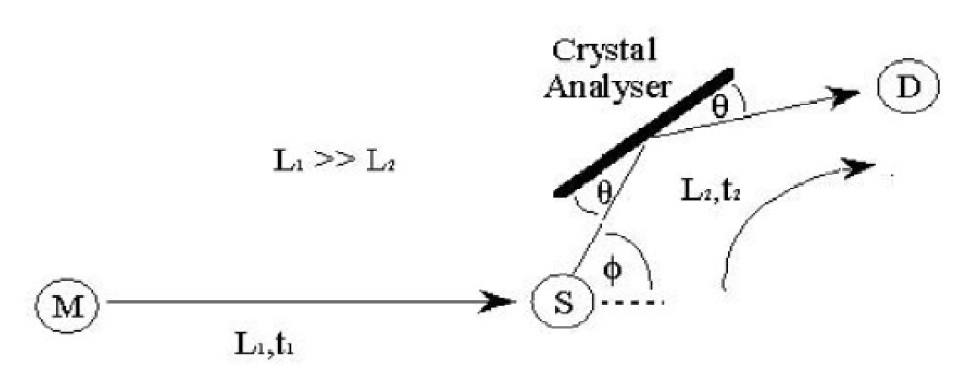
\includegraphics[width=0.6\textwidth]{img/instrument-diagram.png}
\caption{A diagram of an indirect geometry spectrometer. M is the moderator, S is the sample, and D is the detector. $L_1$ is the length of the incident neutron flight path, $L_2$ is the final flight path, $\theta$ is the scattering angle, and $\phi$ is the azimuth angle. In indirect geometry spectrometers the final energy is fixed and is selected using a crystal analyser (typically graphite).}
\label{fig:instrument-diagram}
\end{figure}

Broadly speaking, neutron scattering can be split into two categories:
elastic and inelastic. Elastic scattering is where the final energy of a
scattered neutron is equal to the energy of the incident neutron,
i.e.~there is no transfer of energy to or from the sample. Inelastic
scattering, which is the technique generally used by instruments
belonging to the molecular spectroscopy group (MSG) I was attached to (see section \ref{organisation-of-the-mantid-project-development-team}),
is the more complex case where the energy of the incident neutron and
the scattered neutron are not equal, i.e.~there is a transfer of energy
to or from the sample. From this transfer in energy and from known
parameters of the instrument an instrument independent scattering
function can be defined which provides a full model of the sample. This
function is usually denoted as $S(Q,\omega)$, where $Q$ is the momentum
transfer and $\omega$ is energy transfer {[}3, 4{]}.

\begin{figure}[H]
\centering
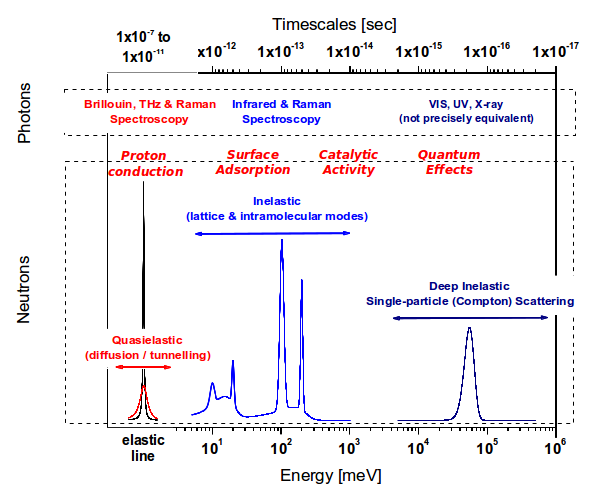
\includegraphics[width=0.6\textwidth]{img/instrument-energy-chart.png}
\caption{Neutron scattering techniques by energy range.}
\label{fig:instrument-energy-chart}
\end{figure}

Two important types of inelastic scattering are quasi-elastic neutron
scattering (QENS) and deep inelastic neutron scattering (a.k.a neutron
Compton scattering). Quasi-elastic neutron scattering is the case where
the energy transfer is very close to zero and the scattering is almost
elastic. This is typically performed on low energy spectrometers such as
IRIS and OSIRIS {[}5, 6{]}. Deep inelastic neutron scattering (DINS) is
the opposite case which uses extremely high energies (\textgreater{}1eV)
and is used to measure the momentum distribution of atoms. This
technique is still in its developmental phase, with the VESUVIO
spectrometer at ISIS currently being the only instrument in the world
capable of DINS {[}7{]}.

Each of the spectrometers used by the MSG are of what is known as
indirect geometry. This is where the final scattered energy is
restricted to a particular wavelength (usually with a analyser crystal
which will absorb all other wavelengths) and the incident neutron energy
is varied. The value of the incident energy can then be found though the
laws of the conservation of energy {[}3{]}.

My work in with the Mantid team was centred round improving and
maintaining the code base for analysis of data from indirect geometry
instruments at ISIS. Mantid includes a framework for loading,
processing and visualising data from the raw time-of-flight
measurements. For a more in-depth introduction to neutron scattering the
reader is directed to the references, in particular refs. {[}3, 4, 8{]}
provide the best introductions to those unfamiliar with the subject.

\clearpage
\section{Organisational Environment}\label{organisational-environment}

\subsection{Organisation of STFC}\label{organisation-of-stfc}

The Science and Technologies Facilities Council (STFC) is a UK based
government funded body that carries out a wide variety of scientific
research across a multitude of disciplines including particle physics,
nuclear physics, space science and engineering, medical and biological
sciences, and computational science. It was formed in 2007 by the merger
of the Particle Physics and Astronomy Research Council (PPARC), the
Council for the Central Laboratory of the Research Councils (CCLRC), and
the Engineering and Physical Sciences Research Council (EPSRC) {[}9{]}.

While the organisation is funded by the government, it is classified as
a non-governmental body which acts as an umbrella organisation for an
array of facilities based across the UK. These include (but are not
limited to) the central laser facility, diamond light source (which is a
publicly limited company of which STFC holds an 86\% share), ISIS
neutron source, and RAL space; all of which are located at Rutherford
Appleton Laboratory in Oxfordshire. The organisation also owns the the
Daresbury Laboratory located in Cheshire and the Chilbolton Observatory
based in Hampshire.

The STFC's head office is located at Polaris House, Swindon, Wiltshire
and is headed by the chief executive John Womersley. The purpose of STFC is
the general organisation and management of the facilities under its
control. In particular it is responsible for allocating budgetary and
staffing allowances and liaising between government departments,
particularly the department for business, innovation and skills which is
the primary government body controlling STFC.

\subsection{Organisation of ISIS Neutron
Source}\label{organisation-of-isis-neutron-source}

ISIS neutron source is a project that is owned, operated and funded by
the STFC. The organisational hierarchy of ISIS is headed by the director
Prof.~Robert McGreevy and includes several division heads for individual
functional areas within ISIS such as the diffraction, spectroscopy and
support, experimental operations, instrumentation, design, and
accelerator divisions.

ISIS is also split into a number of research, operations, and
experimental support groups. The computing group, of which the Mantid
project is a part of, falls into the experimental support group. The
computing group at ISIS is headed by Kevin Knowles. Other members of the
computing group include facilities IT, business applications
development, the ICAT data catalogue, and experimental controls.

While this description provides an overview of how the staffing of ISIS
can be divided, in practice there tends to be a lot of cross over
between sections of the organisation depending on a employee's skills
and responsibilities. For example, while I was employed as part of the
computing group, my line manager and senior manager were both
members of the molecular spectroscopy research group whose interests I
was responsible for within Mantid. However, I still reported to the
Mantid project manager on a daily basis.

\subsection{Organisation of the Mantid Project Development
Team}\label{organisation-of-the-mantid-project-development-team}

The Mantid development team in the UK is a subset of the computing group
of ISIS. The Mantid group is headed by a single project manager (Nick
Draper) who is based at ISIS where the project first started and is
responsible for the overall management and direction of the project. The
project is primarily split into two teams, one based at ISIS and one at the SNS in
Oakridge, Tennessee. Both teams consist of a single lead developer and
several senior developers who oversee the major technical developments
and help to guide and manage the rest of the development team. The US
team also has its own project manager but the project manager based at
ISIS is in overall control.

Within Mantid, the project manager and the majority of the senior
developers are actually contractors from Tessella Ltd. based in
Abingdon, Oxfordshire. The rest of the development team are directly
employed by ISIS, or in the case of the Americans, by the SNS. In
addition there are also several collaborators from facilities such as
the Institut Laue-Langevin (ILL) and the Paul Scherrer Institute (PSI)
who work remotely from their respective facilties.

While I was primarily situated within the development team based at
ISIS, many developers within the team are generally also attached to a
specific scientific group at the facility. In the author's case this was
the ISIS molecular spectroscopy group (MSG) {[}10{]}. The members of the
MSG (and other research groups) are effectively the users of Mantid and
are the people who we gather requirements from, but this is
typically an informal relationship and I worked closely with its
members throughout the year.

\clearpage
\section{Technical and Application
Environments}\label{technical-and-application-environments}

The development team based in the UK has a single office located in the
main office building of the ISIS facility. This office consisted of
approximately 13 workstations. The number of machines varied throughout
the year depending on the level of staffing available to the project.
Each of the machines were reasonably powerful 64-bit Dell workstations
with between 8-16 Gb of RAM and 8-16 core intel i7 processors. Typical
hard drive space for the machines was between 512 Gb to 1 Tb with the
majority still being disk drives, but some of the newer machines had
flash based storage.

The operating system that each machine ran was completely left to the
preference of the developer, but it was recommended that the developer
run one of the operating systems officially supported by Mantid for
obvious reasons. In practice this meant that there was a good variety of
developers using different platforms. I personally chose to run Ubuntu
12.13 as my operating system of choice for the majority of development
work, with a dual partition running Windows 7 which could be swapped to
when circumstances required. Other operating systems used by developers
in the team included Windows 7 \& 8, Mac OSX Mountain Lion and
Mavericks, Red Hat Enterprise Linux 6, and Fedora 20.

Apart from the workstations, the development team also had a collection of
Jenkins build servers in order to support a continuous integration and
testing workflow in conjunction with the Gitflow workflow {[}11{]}. The
build servers are jointly located at both ISIS and the SNS. At the start
of the placement, the build servers for ISIS and the SNS were completely
separate and located at different web address. Each individual build was
run as a single job on the Jenkins build servers. Half way through my
placement this was changed so that the servers were located at the same
web address and the organisation of the build servers was changed to
make use of matrix builds. This is where multiple builds are kicked
off at the same time under a single umbrella job. For example the
development branch matrix build would build the project and run the unit
tests on each officially supported OS every time a new commit was pushed
for integration testing.

Like the choice of operating system, the development software used by
the team was flexible and open to developer preference. The project is
built using the CMake build system on all supported platforms. On
windows platforms the only supported compiler is Visual Studio 2012 or
2014 and most developers either chose to use the Visual Studio IDE, the
Qt Creator IDE, or the Eclipse IDE. On Mac the Intel C++ compiler is
used and typical IDEs are XCode, Eclipse, or Qt Creator. On Linux
distributions the GNU compiler is the main supported compiler, with
either Eclipse or Qt Creator used as the IDE for development. Many Linux
developers are also happy to just use the make command to build the
project from the command line. This approach is often used in
conjunction with lightweight editors such as vim or sublime text. For
interface development, Qt Designer was used on all platforms for
anything more than the most trivial of jobs.

Unit tests are optionally built along side the project using a separate
build target generated by CMake using the CxxTest unit testing
framework. System tests are written in Python and make use of a
collection of custom scripts loosely based on the unittest python module
which makes use of the Mantid Python API. Debugging software used
typically makes use of Visual Studio debugger on Windows, XCode/GDB on
Mac and GDB on Linux distributions.

The Mantid application makes use of data files produced directly from
neutron spectrometers. These files are collected on servers based at
ISIS directly from the instruments themselves and are maintained by the
scientific computing department. These provide both the instrument
scientists and visiting scientists with direct access to the their data.
The development team also has access these servers through network
drives. On Windows operating systems access is provided though the
in-built network drive capabilities. On Mac and Linux access is obtained
through using Samba in conjunction with the SMB protocol. Copies of
actual instrument data are frequently used as part of test scripts,
especially in the case where the data required for the test cannot be
easily simulated programatically.

With regards to project management, the development team makes use of
the git version control system and keeps all of the source code openly
available to the public via Github. The Trac ticketing program is used
to keep a record of the current development progress. The Trac set-up
used also includes plug ins to automatically capture commits to branches
on Github and update the relevant ticket with the commit information.

\clearpage
\section{Description of Job Role and Work
Done}\label{description-of-job-role-and-work-done}

As mentioned in section \ref{organisation-of-the-mantid-project-development-team}, the
majority of my year was spent attached to the Molecular Spectroscopy
Group (MSG) at ISIS. My role in the development team was to satisfy the
computational data analysis requirements of the MSG within Mantid. This
included involvement in every part of the development cycle, from
gathering requirements from the users (the instrument scientists in the
MSG) through to implementation of requested features, to testing and
maintenece/bug fixing.

Before going into discussion about the work I carried out as part of my
placement, it is useful to define a couple of core concepts used within
the Mantid application: algorithms and workspaces. In Mantid a workspace
{[}12{]} is an entity that contains a dataset. There are several types
of workspace, but the most common is a MatrixWorkspace which is a
collection of $n$ X, Y, and E spectra either as a histogram or as point
data. Each spectrum typically corresponds to a single detector but this is
not necessarily always the case. An algorithm {[}13{]} is a class
defined using the the Mantid algorithm framework that manipulates a
workspace in some way (such as loading data into a workspace or
rebinning a workspace). A common analogy is that workspaces are the
`nouns' of Mantid while algorithms are the `verbs'.

\subsection{Initial Training and Development
Work}\label{initial-training-and-development-work}

My first couple of weeks at ISIS were spent running through some
training exercises setup by the development team. These were relatively
simple programming problems designed to gauge my existing understanding
of C++ and Python. After spending a week completing these introductory
activities, I had an informal code review with the lead developer who
examined the good and bad points of what I had written before giving me
an introduction the the Mantid application and workflow of the team. The
following week was mostly spent setting up my workstation for
development before starting my first ticket from the Trac ticket system.
My first ticket involved writing a couple of algorithms which would take
some histogram data and perform smoothing or interpolation of the
workspace using the cubic spline routines in the GSL library, a feature
that had been requested by one of the MSG scientists. From this point
onwards I spent the majority of my time working on tickets for the MSG.

\subsection{Indirect Bayes Interface}\label{indirect-bayes-interface}

Apart from maintenance and minor feature requests my first real major
piece of development work was to write a GUI for a collection of
Bayesian fitting routines that had been provided by one of the
scientists in the group. These routines are used as part of
quasi-elastic neutron scattering analysis to determine the shape of the
scattering function present in the dataset by using Bayesian methods to
compute the likelihood of a given model. These methods are based on the
original routines described by Sivia {[}14{]}.

\begin{figure}[H]
\centering
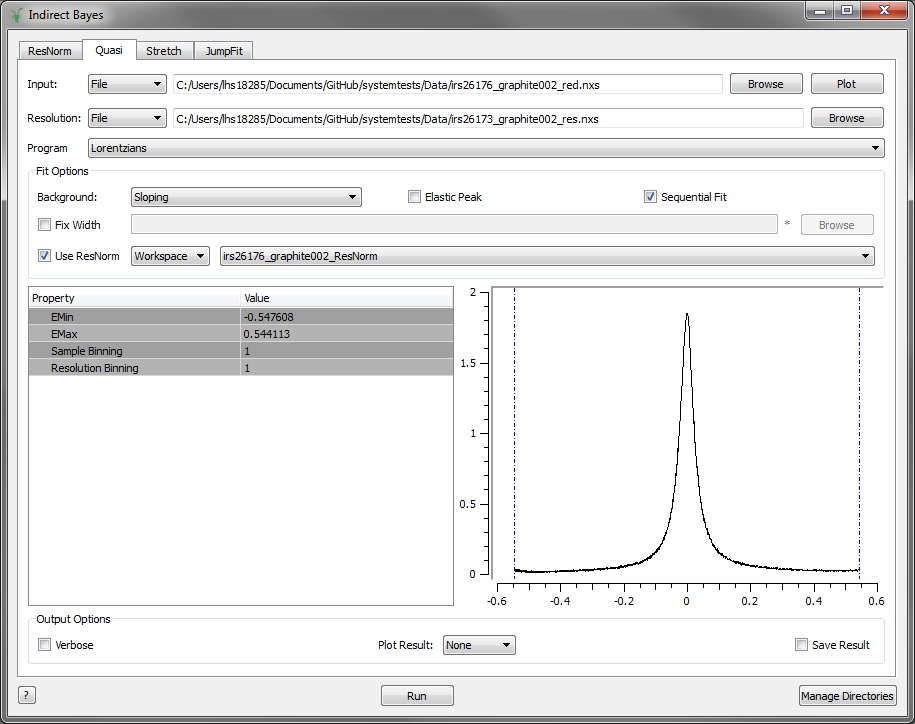
\includegraphics[width=0.6\textwidth]{img/iris-bayes-quasi.png}
\caption{Screen capture of the Indirect Bayes QENs analysis interface in Mantid.}
\label{fig:bayes-gui}
\end{figure}

The purpose of the interface was to provide an easier way for users to
set up and run a fit to their data than by using the existing scripts
which required many parameters to be specified. This was fiddly and
often led to the user inputting incorrect combinations of parameters
causing the script to throw an error or even crash Mantid.

The solution to this was to add another custom interface under the
indirect section of the application (there where already three others in
place). This consisted of a collection of C++ classes, created using the
Qt framework, one for the parent window of the GUI and one for each of
the individual routines on the interface which were implemented as
separate tabs on the interface. Each of the routines were refactored
from the original code base and required updated system tests, which
were implemented at the same time as the new interface.

\subsection{VESUVIO Calibration}\label{vesuvio-calibration}

Another major piece of work I was involved with during my placement was
porting some calibration scripts for the VESUVIO instrument {[}7{]} which were
originally written as Fortran programs for the older OpenGenie
application {[}15{]}. As part of this project, I created a new
implementation for Mantid based on the original calibration procedures
described in ref. {[}16{]}.

This required rigorous testing by the scientist responsible for the
instrument and was built slowly over several of months. The Mantid
implementation was designed to be radically different from the original.
The new version was built using the Mantid concepts of algorithms and
workspaces and was intended to be more maintainable than the original. I
also wrote a couple of unit test suites used to check the quality of the
calibration using several different sample materials at the same time.

\begin{figure}[H]
\centering
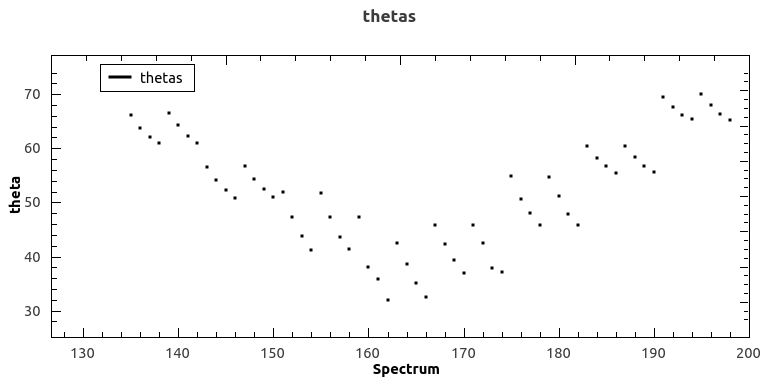
\includegraphics[width=0.6\textwidth]{img/calib-theta.png}
\caption{Plot of the calibrated values for $\theta$ from a Pb sample output from the VESUVIO calibration program. Compare this with the $\theta$ plots in reference {[}16{]}.}
\label{fig:calib-theta}
\end{figure}

The end product was a pair of Mantid algorithms, one for fitting the
appropriate line shape to each peak in every spectrum of a sample run
specifcially measured for calibration with the Mantid python API and one
which calculated the calibration parameters for the instrument using the
parameters of the fit obtained from the first algorithm.

\subsection{Density of States
Algorithm}\label{density-of-states-algorithm}

During my time with the MSG, it became apparent that one of the major
areas for development that had not been explored was the implementation
of support for the simulation of a neutron scattering experiment. This
was an area which my supervisor within the MSG (who has a background in computational
simulations) was keen to expand because comparison with simulation is
one of the most common and useful techniques for analysing experimental
data.

One of her requests was to add support in Mantid for loading the results
of a simulation produced using the CASTEP code {[}17{]}. My supervisor
already had a perl script which could do the calculations she required
through the command line, but it was infinitely more convenient to have
this functionality within Mantid.

This involved the creation of a new algorithm which would read the files
output from CASTEP, which contained a list of frequencies predicted by
theory for a sample. With this information, the density of states could
be calculated and a workspace containing the simulated spectrum could be
created. Functionality was also added to calculate the infrared and
Ramen spectra from data in the files. Later in the placement she requested additional functionality be added to the algorithm to
calculate the partial density of states from CASTEP code.

\hyperdef{}{improvements-to-algorithm-history-recording}{\subsection{Improvements
to Algorithm History
Recording}\label{improvements-to-algorithm-history-recording}}

Occasionally I became involved in the more general development of the
Mantid framework. The largest piece of general development I was asked
to do was to improve the algorithm history system. In Mantid, when
algorithms get executed on a workspace a record of the algorithm run and
the parameters used to execute the algorithm are stored on the workspace
object. In theory this can provide a detailed record of everything that
has happened to the workspace from the moment the data entered the
application. In practice this feature had only been partially
implemented and had slowly become more redundant/broken as development
moved on.

\begin{figure}[H]
\centering
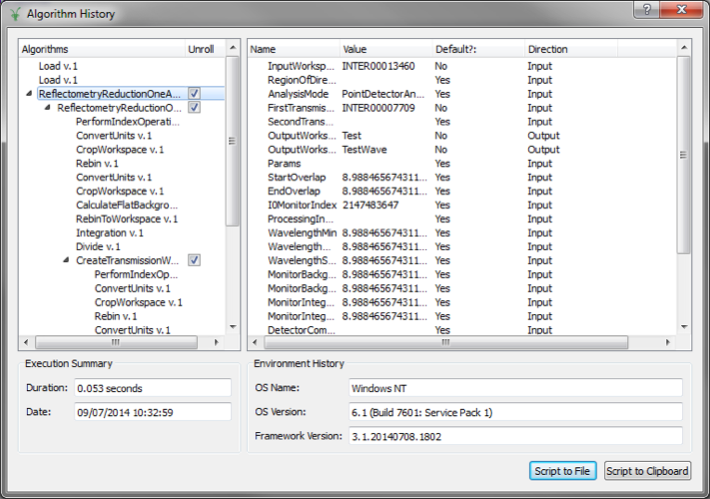
\includegraphics[width=0.6\textwidth]{img/algorithm-history.png}
\caption{Screen capture of the algorithm history GUI showing nested algorithms used on a workspace from the INTER spectrometer.}
\label{fig:algorithm-history}
\end{figure}

My task was to overhaul this feature to not only properly provide the
features mentioned above, but also to add functionality to capture
nested algorithm history, that is, the history of an algorithm operating
on a workspace but also the history of an `child' algorithms run as part
of that algorithm. There was also a requirement to make the workspace
completely reproducible from its history alone and that the full nested
history could be examined using a GUI from within Mantid.

As this consisted mostly of core system changes a much more rigorous
design phase was required. A draft of a design document already existed
for the algorithm history which I presented to the development team
(both in the UK and the states) and was roundly rejected for being too
vague. The next step was go prototype out some of the more unclear
features such as how history should be saved to file which needed to be
a compromise space and time efficiency, how to represent nested history
at runtime (e.g. boost::graph, std::list of children, std::set of children?),
and how nested history records should be stored on disk.

After prototyping the system, I created a new design document with the
findings from the prototypes and my suggested proposals for change
{[}18{]}. This document was reviewed by the senior members of the
development team and with a few minor changes was approved. I then spent
the next month or so implementing the changes outlined in the design
document. Along the way we encountered several issues that were not
covered by the design document, mostly linked technical issues caused by
the fact that workspaces can be created without a string name and that
that providing a temporary name to them on the fly can causes many
issues with reproducing a executable script.

Despite these set backs, I managed to get the majority of the core
changes into Mantid in time for the next release. However there were
still several parts of the system left to the next release cycle, such
compressing the size of large algorithm properties (such as when arrays
are passed as parameters to an algorithm), which was left to my
successor.

\subsection{Development Reports}\label{development-reports}

One final piece of work I was ask to complete during my time at ISIS was
to produce two major reports. The first {[}19{]} was to provide a snapshot of the
current progress of development of the indirect framework. This report
gives an overview of the entire framework as of release 3.1 including a
description of the theory behind the routines and detailed description
of how each one works. Suggested ideas for future development are also
listed.

The second report {[}20{]} was a basic user manual for the routines still under
development for the VESUVIO spectrometer and provides a description of
how to analyse data from the instrument with the implementation as it
stands. Both of these reports are publicly available for free via the RAL ePubs system.

\clearpage
\section{Critical Evaluation of
Placement}\label{critical-evaluation-of-placement}

My overall experience with the placement was a positive one. ISIS provided me with a level of responsibility far exceeding
anything I expected. For the most part, I felt that I was a valued member
of the development team and that I was treated as an equal rather than
as an intern. I feel that my practical understanding of software
development has increased tenfold, particularly over the first few
months which I found to be a steep but enjoyable learning curve. I left
the placement feeling much more technically proficient and
professionally competent than when I finished the second year of my
course.

One of the first things that I learned when I started the placement was
how to read other peoples code and how to mentally navigate a large code
base. While these skills may seem trivial to the established developer I
found that they only be gained by exposure to a large project with multiple developers.

When I started the placement I had only taken a single module in C++ and
I was self taught to the beginner level in Python. After a year of being
heavily exposed to both languages, I feel confident enough to call
myself an intermediate in both languages. Besides gaining a better
understanding of new languages though constant exposure, I have also
gained experience with a variety of supporting libraries and tools. For
example, I had not worked with the boost library before my placement
which was used extensively through out the project to provide C++11 like
features in a cross platform and backwardly compatible way. I have become much more adept at using
development tools such as Git, GDB, CMake, and Valgrind which I had
little or no experience with previously.

Beyond enhancing my technical knowledge the placement has also provided
me with great opportunities to better my `soft skills'. Over the course
of the 14 months I spent at RAL, we released a new version of Mantid 4
times. At three of the releases I was asked to present what I had been
working on to the ISIS faculty which mainly consisted of instrument
scientists with limited knowledge of the development process. The content of what I presented varied, but I usually
presented any changes to the indirect inelastic section, but I also
presented more general topics on occasion (such as the algorithm history
changes, see section on
\ref{improvements-to-algorithm-history-recording}). I was also asked to present directly to
the MSG during one of their monthly meetings and to present any core
changes to Mantid during their biweekly development meetings. As I would
not describe myself as a natural speaker, opportunities to present
material to a variety of different audiences (both in size and
demographic) proved to invaluable experience.

Talking to and gathering requirements from users was another skill that
felt I developed well over the course of the year. I met with members of
the MSG on a regular basis to pin down the requirements of the group. I
also frequently encouraged MSG members to contact me if they had any
features or bug fix requests, many of whom did. This allowed me to
quickly build a solid relationship with the scientists in the group who
would regularly contact me with feedback on their experiences with the application. Being an informal working
environment, requirements gathering generally consisted of going to the relevant person's office with a notepad
and having a short chat about any issues/feature requests, before going
anyway and implementing the requests and getting it into the nightly
build for them to play with. I felt that generally this system worked
quite well. Users in many cases users could physically show me the
issues they were having and it was faster than emailing back a forth. I
felt this approach of regular contact also broke down the ``them and
us'' wall between scientists and the development team.

Despite these many positive aspects there were several low points to
the placement that I felt could of been improved upon. While the
development team I worked with was for the most part friendly and
helpful I found that there appeared to be a lack of cohesion within the
group. Team members seemed to work fairly independently of one another
in their own areas which seemed to cause a diversion of goals and a lack
of communication which manifested itself as defects in the project. Most
of the GUIs for individual experimental techniques are completely
different from one another (not just in function, but in look and feel
and GUI conventions). I felt that the development team could of
benefitted from some basic team building activities or even the
occasional social activity to try and build teamwork and get them
talking to one another. I believe that the Mantid team was the only
group at RAL who didn't have coffee breaks together!

Leading on from this point I noticed over the course of the year that
there appeared to be project divergence between the American development
team and the UK development team. It is worth noting that the
instruments based at the SNS primarily use event data (where each
individual neutron detection event is recorded indivudually) while ISIS
mostly uses histogram data, which means that there fundamentally must be
some difference between the two. However, as with individual techniques,
there appears to be a completely different line of development
undertaken for the Americans, with their own separate GUIs and routines,
much of which could potentially be combined. Again, I believe this was
down to a communication problem. The both teams only had a single
biweekly development meeting via BlueJeans (which often got cancelled)
and an ongoing Skype IM conversation as the means to contact one
another. This meant that the people on both sides of the atlantic would
often not communicate for days or weeks at a time.

I feel the simplest solution to this issue would be to increase the
number of opportunities that members on both sides of the atlantic have
to talk to one another. I would suggested upping the number of code
reviews (at least one a week) and having a daily standup meeting with
both sides in attendance over BlueJeans. I think this would help to keep
both development teams better informed of the general direction of the
project.

I also found there to be several issues in the specific area I was
working in. The quality of the code base underlying the indirect
geometry framework of Mantid was generally poor. There was only minimal
coverage of the code base with system tests and zero unit tests. A lot
of the underlying Python scripts and Fortran routines had been written
by scientists and were not of production quality and no attempt had been
made to refactor the code before integrating it into the Mantid
framework. Docstrings, commenting and documentation was almost
non-existent. I believe this was caused by years of placement students being left to look after the section on there own, some of whom were obviously less competent than others, resulting in disorganised and fractured code base.

This proved to be incredibly difficult to work with. Large portions of
my time were spent re-writing code to make it more reusable,
maintainable, and better documented. When receiving new scripts from
scientists I would aggressively refactor it and pester the writer for
documentation of why the routine was useful and what it does
(particularly if they could produce a paper outlining the method). I
also began to write unit tests and system tests for any new routines.
While the code base was still no where near the level of quality I would
expect by the time I left, I did feel that these measures were slowly
starting to make an impact on the quality of the code. This taught me that unit tests give a developer confidence to make changes and how to refactor properly.

Finally, one further negative issue I had to deal with on several
occasions was a lack of direction and the conflict of interest between
developers and instrument scientists. Several of the scientists within
my group approached me to request features that they would like to see
or to suggest improvements. This is good because it means we write what
the use wants, but can become burdensome when there is a lack of
prioritisation. I often found myself `spinning many plates' for many
different task masters. Occasionally this led to a conflict either
between what individual scientists want or between what scientists want
and the general goals of the project.

Towards the end of the year I felt we began to rectify this by having a
weekly meeting where myself, my line manager (an MSG scientist) and a
retired scientist who's profession was QENs data analysis along with
guests from both the development team and the scientific group. This
allowed us to better outline what our goals should both in the short an
long term, as well as increasing communication between all parties.

All of these issues really outlined to me the importance of good communication within a development team. While these issues were not so horrendous as to prevent the team from delivering the software, I really felt that even the smallest amount of miscommunication can lead to bad engineering and long delays.

In summary, I feel that I had an excellent placement a ISIS. I was given
responsibilities above and beyond anything I had imagined before
starting my industrial year. I met and worked with some very interesting
people and an worked for unusual company. The learning curve was the
steepest I've ever experienced, but I enjoyed every moment. Despite
several negative aspects to the project and making many mistakes along
the way, I feel that I was able to learn from them all.

\section*{Bibilography}\label{bibilography}
\addcontentsline{toc}{section}{Bibilography}

{[}1{]} ISIS Neutron Source, ``How ISIS works.''
\url{http://www.isis.stfc.ac.uk/about/how-isis-works6313.html},
May-2014.

{[}2{]} Mantid Project, ``Mantid: Manipulation and analysis toolkit for
instrument data,'' 2013 {[}Online{]}. Available:
\url{http://dx.doi.org/10.5286/SOFTWARE/MANTID}

{[}3{]} D. S. Sivia, \emph{Elementary scattering theory for x-ray and
neutron users}. OUP Oxford, 2011.

{[}4{]} F. Fernandez-Alonso and D. L. Price, \emph{Neutron scattering
fundermentals}, 1st ed. Academic Press, 2013.

{[}5{]} V. Garcia-Sakai, M. Adams, W. Howells, and M. Telling, ``The
IRIS user guide,'' Rutherford Appleton Laboratory UK, RAL-TR-2011-004,
2011.

{[}6{]} M. Telling and K. Andersen, ``The OSIRIS user guide,''
Rutherford Appleton Laboratory UK, RAL-TR-2003-016, 2003.

{[}7{]} J. Mayers and G. Reiter, ``The VESUVIO electron volt neutron
spectrometer,'' \emph{Measurement Science and Technology}, vol. 23, no.
4, p. 045902, 2012.

{[}8{]} R. Pynn, ``Neutron scattering: A non-destructive microscope for
seeing inside matter,'' in \emph{Neutron scattering applications and
techniques}, Springer, 2008.

{[}9{]} House of Commons Science and Technology Committee, ``Office of
science and innovation: Scrutiny report 2005 and 2006.'' ISBN
0-215-03350-7, 2007.

{[}10{]} ISIS Neutron Source, ``Molecular spectroscopy group.''
\url{http://www.isis.stfc.ac.uk/groups/molecular-spectroscopy/molecular-spectroscopy-3384.html},
May-2014.

{[}11{]} Mantid Project, ``Git workflow.''
\url{http://www.mantidproject.org/Git_Workflow}, August-2014.

{[}12{]} Mantid Project, ``Workspace.''
\url{http://www.mantidproject.org/Workspace}, August-2014.

{[}13{]} Mantid Project, ``Algorithms.''
\url{http://www.mantidproject.org/Algorithm}, August-2014.

{[}14{]} D. Sivia, C. Carlile, W. Howells, and S. K{ö}nig, ``Bayesian
analysis of quasielastic neutron scattering data,'' \emph{Physica B:
Condensed Matter}, vol. 182, no. 4, pp. 341--348, 1992.

{[}15{]} Open Genie, ``Open genie homepage.''
\url{http://www.opengenie.org/Main_Page}, August-2014.

{[}16{]} J. Mayers and M. Adams, ``Calibration of an electron volt
neutron spectrometer,'' \emph{Nuclear Instruments and Methods in Physics
Research Section A: Accelerators, Spectrometers, Detectors and
Associated Equipment}, vol. 625, no. 1, pp. 47--56, 2011.

{[}17{]} CASTEP, ``CASTEP homepage.'' \url{http://www.castep.org},
September-2014.

{[}18{]} Github, ``Mantid project: Nested history detailed design
document.''
\url{https://github.com/mantidproject/documents/blob/master/Design/Nested\%20History\%20Detailed\%20Design\%20Document.docx},

{[}19{]} S. Jackson, ``An overview of the recent development of indirect inelastic data analysis in Mantid,''
Rutherford Appleton Laboratory UK, RAL-TR-2014-010, 2014.
September-2014.

{[}20{]} S. Jackson, ``VESUVIO Data Reduction and Analysis in Mantid,''
Rutherford Appleton Laboratory UK, RAL-TR-2014-009, 2014.
September-2014.
\end{document}
